\documentclass[12pt]{beamer}
\usetheme[whale]{Hannover}
\usepackage[utf8]{inputenc}
\usepackage{subfig}
\usepackage{graphicx}
\usepackage{listings}
\usepackage{capt-of}
\title{Web-basierte Registrierkasse}
\author{Lukas Gritsch Benjamin Cilga}

\renewcommand{\figurename}{Bild}

\begin{document}

\setbeamertemplate{section in toc}{\inserttocsection}

\begin{frame}[plain]
\maketitle
\small
\end{frame}

\begin{frame}
	\tableofcontents
\end{frame}


\section{Praktische Ausarbeitung und Programmierung}

\begin{frame}
	\begin{Large}
		\begin{center}
			Praktische Ausarbeitung und Programmierung
		\end{center}
	\end{Large}
\end{frame}


\begin{frame}
\frametitle{Übersicht}
\Large Funktionsweise
\begin{figure}[h]
	\centering
	\subfloat[MVC-Pattern]{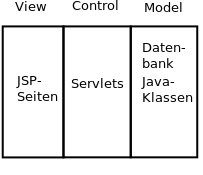
\includegraphics[scale=0.55]{Bilder/MVC.png}} \hfill
	\subfloat[Modell]{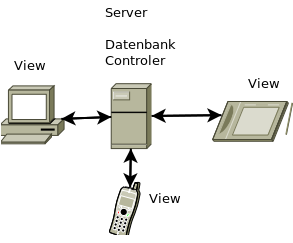
\includegraphics[scale=0.45]{Bilder/Modell.png}}
	
\end{figure}
\end{frame}

\subsection{Einarbeitungsphase}

\subsubsection{Laravel}

\begin{frame}
\frametitle{Laravel}

\begin{Large}
Grobe Fakten \vspace{0.2 cm}
\end{Large} 

\begin{itemize}
	\item[-] PHP Framework
	\item[-] Arbeitet nach dem MVC Prinzip (Pattern)
	\item[-] Übernimmt Datenbankverwaltung  
	\item[-] Quellcode wird sehr stark vereinfacht
\end{itemize}
	
\end{frame}


\subsubsection{Servlets und JSP Dateien}

\begin{frame}
	\frametitle{Servlets und JSP Dateien}
	
	\begin{Large}
		Grobe Fakten \vspace{0.2 cm}
	\end{Large}		
	\begin{itemize}
		\item[-] Java und HTML code
		\item[-] Folgt keinen spezifischen Prinzip (Pattern), es wird aber auch meist nach MVC gearbeitet
		\item[-] Logik für die Datenbankverwaltung muss selbst erstellt werden
		
	\end{itemize}
	
\end{frame}


\subsection{Umsetzungsphase}
\begin{frame}
\frametitle{Umsetzungsphase}

\begin{Large}
Herausforderung Rechnungserstellung \vspace{0.2 cm}
\end{Large}

\begin{itemize}
	\item[-] Verwendung von \LaTeX \hspace{0.05 cm} zum Erstellen der Rechnung
	\item[-] Probleme mit dem Kompilieren der Rechnung
	\item[-] Daten wurden in falschem Verzeichnis gespeichert
\end{itemize}

\end{frame}




\subsection{Testphase}

\begin{frame}
\frametitle{Testphase}

\begin{Large}
	Rasperry Pi als Testserver \vspace{0.2 cm}
\end{Large}
	\begin{itemize}
		\item[-] Verwendung von raspbian-jessie (Debian Distribution)
		\item[-] Installation von Tomcat 
		\item[-] Übertragen der .war Datei in das Tomcat Verzeichnis 
	\end{itemize}
\end{frame}

\subsubsection{Testdurchlauf}

\begin{frame}
	Finden des Rasperry Pi im Heimnetzwerk
	\begin{figure}
		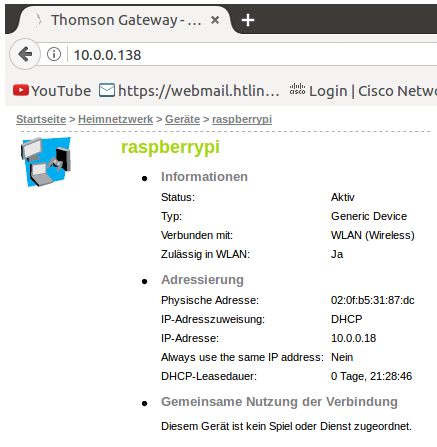
\includegraphics[scale=0.46]{Bilder/gatewayInt.png}
		\caption{Resparry Pi Informationen am Gateway}
	\end{figure}		
\end{frame}

\begin{frame}
	Aufrufen der Anwendung im Web-Browser
	
	\begin{figure}
		
\includegraphics[scale=0.7]{Bilder/url.png}
	\end{figure}
	\begin{figure}
		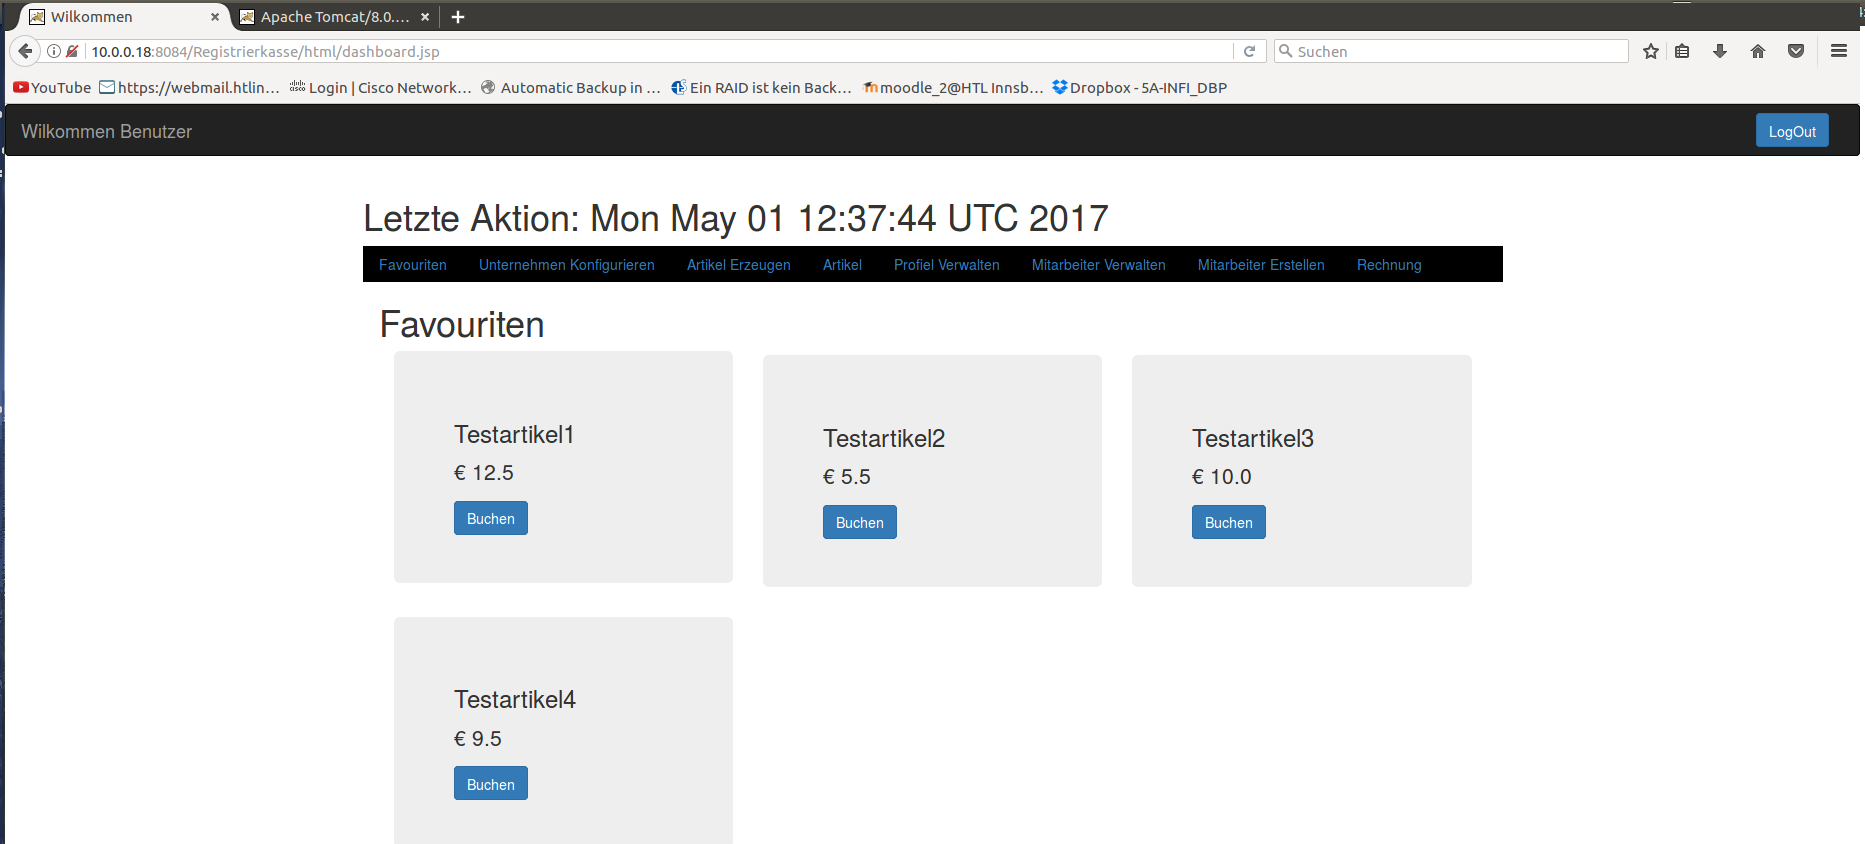
\includegraphics[scale=0.13]{Bilder/favouriten.png}
		\caption{Erscheinung nach dem Login}
	\end{figure}
\end{frame}

\begin{frame}
Erstellen der Rechnung
\begin{figure}
	
\includegraphics[scale=0.5]{Bilder/URL1.png}
\end{figure}
\begin{figure}
	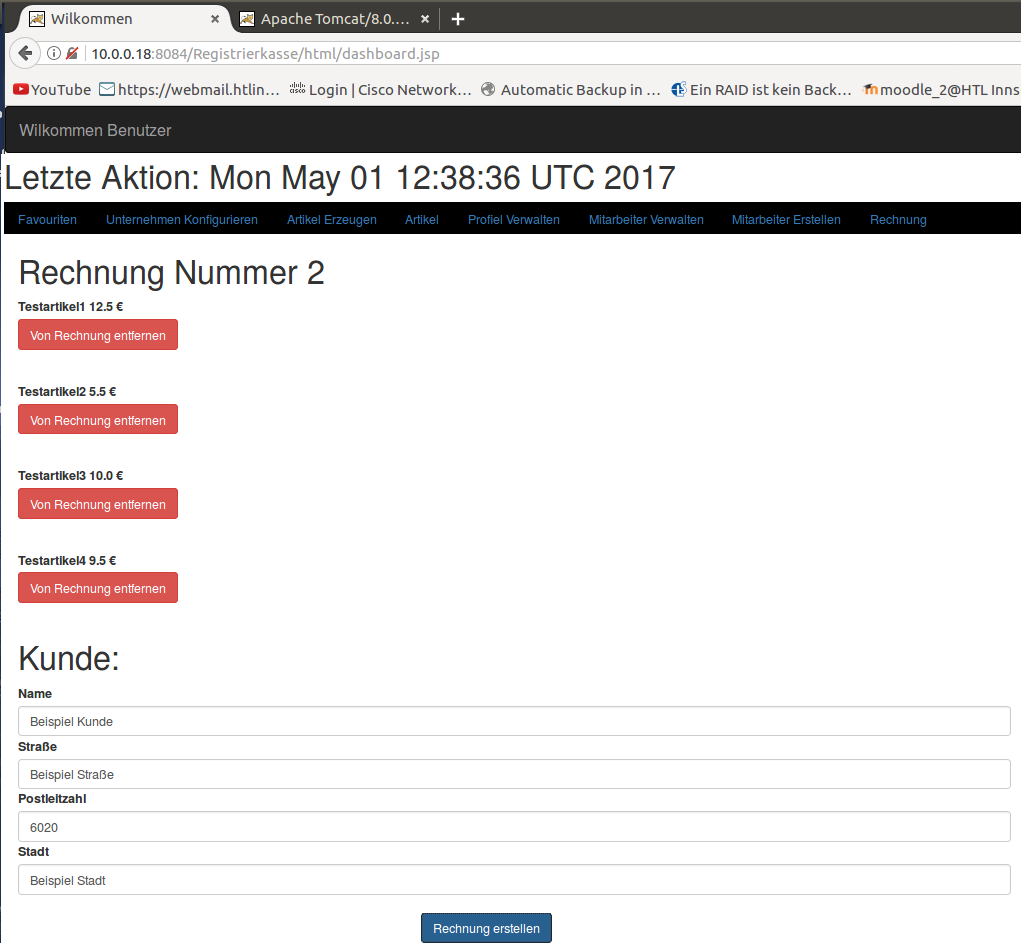
\includegraphics[scale=0.17]{Bilder/rechnungErstellen.png}
	\caption{Erstellen der Rechnung}
\end{figure}

\end{frame}

\begin{frame}
	Rechnung herunterladen oder drucken
	\begin{figure}
		
\includegraphics[scale=0.5]{Bilder/URL2.png}
\end{figure}		
	
	\begin{figure}
		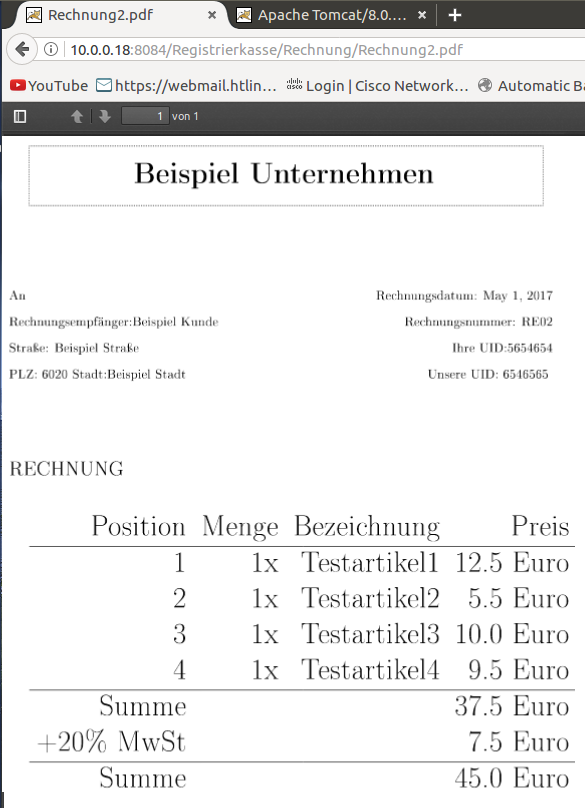
\includegraphics[scale=0.2]{Bilder/rechnung.png}
		\caption{Rechnung Herunterladen oder Drucken }
\end{figure}		
	
\end{frame}


\begin{frame}
	\begin{Large}
		\begin{center}
				Vielen Dank für Ihre Aufmerksamkeit !
		\end{center}
	\end{Large}
\end{frame}


\begin{frame}
	\begin{Large}
		\begin{center}
			Wirtschaftliche Ausarbeitung
		\end{center}
	\end{Large}
\end{frame}

\section{Wirtschaftliche Ausarbeitung}
\subsection{Marktforschung}
\begin{frame}
\frametitle{Marktforschung}
\begin{itemize}
\item Ziel: Ausschlaggebende Eigenschaften einer Registrierkassensoftware feststellen (für Konkurrenzanalyse)
\item wurde mittels Fragebögen durchgeführt
\item 1.Fragebogen: Wichtige Eigenschaften einer Registrierkassensaftware feststellen
\item 2.Fragebogen: Diese Eigenschaften nach ihrer Wichtigkeit anordnen
\end{itemize}
\end{frame}
\begin{frame}
\frametitle{Marktforschung}
Ergebnis
\begin{itemize}
\item Funktionalität: 13 Punkte
\item Laufsicherheit: 15 Punkte
\item Preis: 17 Punkte
\item Bedienbarkeit/Benutzerfreundlichkeit: 17 Punkte
\item Hardwareunabhängigkeit: 21 Punkte
\item Übersichtlichkeit: 22 Punkte
\item andere: 35 Punkte
\end{itemize}
\end{frame}
\subsection{Konkurrenzanalyse}
\begin{frame}
\frametitle{Konkurrenzanalyse}
\begin{itemize}
\item Ziel: Determinieren ob ein Eintritt in den Markt sinnvoll wäre, Festellen ob der Markt weiter unterteilt werden kann
\item Konkurrenten wurden anhand ihrer Relevanz priorisiert (Google)
\item Methodik des Stärken-Schwächen-Profils wurde verwendet
\end{itemize}
\end{frame}
\begin{frame}
\frametitle{Konkurrenzanalyse}
\begin{figure}
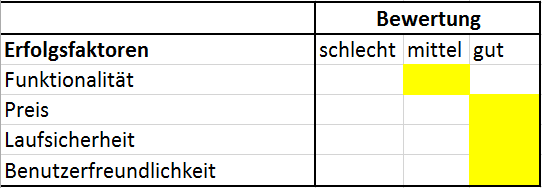
\includegraphics[scale=0.6]{Bilder/Idealprofil}
\caption{Idealprofil}
\end{figure}
\end{frame}
\begin{frame}
\frametitle{Konkurrenzanalyse}
Ergebnis:
\newline
\begin{itemize}
\item Eintritt in den Markt ist nicht sinnvoll
\item Der Markt kann nicht weiter segmentiert werden
\end{itemize}
\end{frame}
\subsection{Break-Even-Point-Analyse}
\begin{frame}
\frametitle{Break-Even-Point-Analyse}
\begin{itemize}
\item Ziel: Determinieren wann sich der Absatz dieser Registrierkassensoftware rentieren würde
\item Kosten: Entwicklungskosten, Serverbetriebskosten
\item Break-Even-Point: Alle Kosten gedeckt und Einkommen gegeben
\end{itemize}
\end{frame}
\begin{frame}
\frametitle{Break-Even-Point-Analyse}
\begin{figure}
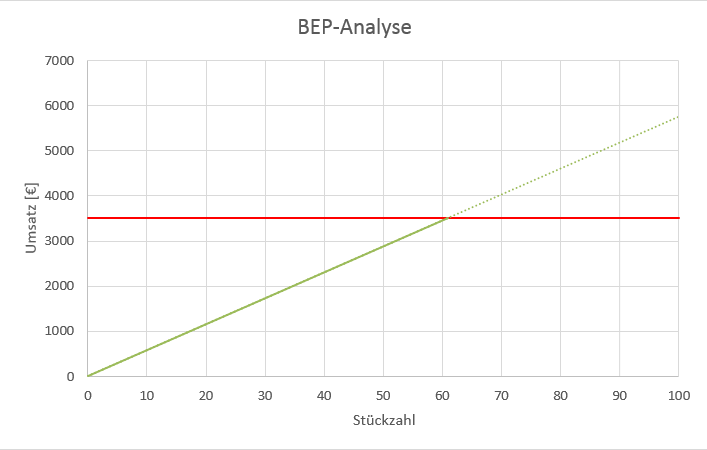
\includegraphics[scale=0.45]{Bilder/BEP}
\end{figure}
\end{frame}

\begin{frame}
	\begin{Large}
		\begin{center}
				Vielen Dank für Ihre Aufmerksamkeit !
		\end{center}
	\end{Large}
\end{frame}
\end{document}
